\documentclass[conference,final]{IEEEtran}

\usepackage[colorlinks]{hyperref}
\usepackage[normalem]{ulem}
\usepackage[utf8]{inputenc}
\usepackage{amsmath}
\usepackage{amssymb}
\usepackage{booktabs}
\usepackage{color}
\usepackage{fancyvrb}
\usepackage{float}
\usepackage{graphicx}
\usepackage{ifpdf}
\usepackage{keyval}
\usepackage{listings}
\usepackage{moresize}
\usepackage{multirow}
\usepackage{rotating}
\usepackage{setspace}
\usepackage{subfigure}
\usepackage{url}
\usepackage{wrapfig}
\usepackage{xcolor}
\usepackage{xspace}

\definecolor{listinggray}{gray}{0.95}
\definecolor{darkgray}{gray}{0.7}
\definecolor{commentgreen}{rgb}{0, 0.4, 0}
\definecolor{darkblue}{rgb}{0, 0, 0.4}
\definecolor{middleblue}{rgb}{0, 0, 0.7}
\definecolor{darkred}{rgb}{0.4, 0, 0}
\definecolor{brown}{rgb}{0.5, 0.5, 0}

\makeatletter
\def\cyanuwave{\bgroup \markoverwith{\lower3.5\p@\hbox{\sixly \textcolor{cyan}{\char58}}}\ULon}
\def\reduwave{\bgroup \markoverwith{\lower3.5\p@\hbox{\sixly \textcolor{red}{\char58}}}\ULon}
\def\blueuwave{\bgroup \markoverwith{\lower3.5\p@\hbox{\sixly \textcolor{blue}{\char58}}}\ULon}
\font\sixly=lasy6
\makeatother

\AtBeginDocument{
  \hypersetup{
    citecolor=blue,
    linkcolor=blue,   
    urlcolor=blue}}
\newif\ifdraft
\drafttrue
\ifdraft
\definecolor{ocolor}{rgb}{1,0,0.4}
\newcommand{\onote}[1]{ {\textcolor{ocolor} { (***Ole: #1) }}}
\newcommand{\terminology}[1]{ {\textcolor{red} {(Terminology used: \textbf{#1}) }}}
\newcommand{\owave}[1]{ {\cyanuwave{#1}}}
\newcommand{\jwave}[1]{ {\reduwave{#1}}}
\newcommand{\alwave}[1]{ {\blueuwave{#1}}}
\newcommand{\jhanote}[1]{ {\textcolor{red} { ***shantenu: #1 }}}
\newcommand{\alnote}[1]{ {\textcolor{blue} { ***andreL: #1 }}}
\newcommand{\amnote}[1]{ {\textcolor{blue} { ***andreM: #1 }}}
\newcommand{\georgenote}[1]{ {\textcolor{brown} { ***sharath: #1 }}}
\newcommand{\revThreeNote}[1]{ {\textcolor{purple}{}}} 
\newcommand{\revOneNote}[1]{ {\textcolor{purple}{}}} 
\newcommand{\revTwoNote}[1]{ {\textcolor{purple}{}}} 
\definecolor{orange}{rgb}{1,.5,0}
\newcommand{\aznote}[1]{ {\textcolor{orange} { ***ashley: #1 }}}
\definecolor{dandelion}{cmyk}{0,0.29,0.84,0}
\newcommand{\mtnote}[1]{ {\textcolor{dandelion} { ***matteo: #1 }}}
\newcommand{\note}[1]{ {\textcolor{magenta} { ***Note: #1 }}}
\else
\newcommand{\onote}[1]{}
\newcommand{\terminology}[1]{}
\newcommand{\owave}[1]{#1}
\newcommand{\jwave}[1]{#1}
\newcommand{\alnote}[1]{}
\newcommand{\amnote}[1]{}
\newcommand{\athotanote}[1]{}
\newcommand{\georgenote}[1]{}
\newcommand{\pmnote}[1]{}
\newcommand{\jhanote}[1]{}
\newcommand{\msnote}[1]{}
\newcommand{\mrnote}[1]{}
\newcommand{\aznote}[1]{}
\newcommand{\mtnote}[1]{}
\newcommand{\note}[1]{}
\newcommand{\revOneNote}[1]{}
\newcommand{\revTwoNote}[1]{}
\newcommand{\revThreeNote}[1]{} 
\fi

\newcommand{\cloud}{cloud\xspace}
\newcommand{\clouds}{clouds\xspace}
\newcommand{\pilot}{Pilot\xspace}
\newcommand{\pilots}{Pilots\xspace}
\newcommand{\pilotjob}{Pilot-Job\xspace}
\newcommand{\pilotjobs}{Pilot-Jobs\xspace}
\newcommand{\pilotcompute}{Pilot-Compute\xspace}
\newcommand{\pilotcomputedescription}{Pilot-Compute Description\xspace}
\newcommand{\pilotdescription}{Pilot-Description\xspace}
\newcommand{\pilotcomputes}{Pilot-Computes\xspace}
\newcommand{\pilotdata}{Pilot-Data\xspace}
\newcommand{\pilotdatainmem}{Pilot-Data Memory\xspace}
\newcommand{\pilotdatadescription}{Pilot-Data Description\xspace}
\newcommand{\pilotdataservice}{Pilot-Data Service\xspace}
\newcommand{\pilotcomputeservice}{Pilot-Compute Service\xspace}
\newcommand{\computedataservice}{Compute-Data Service\xspace}
\newcommand{\computedatamanager}{Compute-Data Manager\xspace}
\newcommand{\computeunitdescription}{Compute-Unit Description\xspace}
\newcommand{\dataunitdescription}{Data-Unit Description\xspace}
\newcommand{\pilotmapreduce}{PilotMapReduce\xspace}
\newcommand{\mrmg}{MR-Manager\xspace}
\newcommand{\pstar}{P*\xspace}
\newcommand{\pd}{PD\xspace}
\newcommand{\pc}{PC\xspace}
\newcommand{\pcs}{PCs\xspace}
\newcommand{\pj}{PJ\xspace}
\newcommand{\pjs}{PJs\xspace}
\newcommand{\pds}{Pilot Data Service\xspace}
\newcommand{\computeunit}{Compute-Unit\xspace}
\newcommand{\computeunits}{Compute-Units\xspace}
\newcommand{\dataunit}{Data-Unit\xspace}
\newcommand{\dataunits}{Data-Units\xspace}
\newcommand{\du}{DU\xspace}
\newcommand{\dus}{DUs\xspace}
\newcommand{\dud}{DUD\xspace}
\newcommand{\cu}{CU\xspace}
\newcommand{\cus}{CUs\xspace}
\newcommand{\cud}{CUD\xspace}
\newcommand{\su}{SU\xspace}
\newcommand{\sus}{SUs\xspace}
\newcommand{\schedulableunit}{Schedulable Unit\xspace}
\newcommand{\schedulableunits}{Schedulable Units\xspace}
\newcommand{\cc}{c\&c\xspace}
\newcommand{\CC}{C\&C\xspace}
\newcommand{\up}{\vspace*{-1em}}
\newcommand{\upp}{\vspace*{-0.5em}}
\newcommand{\numrep}{8 }
\newcommand{\samplenum}{4 }
\newcommand{\tmax}{$T_{max}$ }
\newcommand{\tc}{$T_{C}$ }
\newcommand{\tcnsp}{$T_{C}$}
\newcommand{\bj}{BigJob\xspace}
\newcommand{\irods}{iRODS\xspace}

\newcommand{\I}[1]{\textit{#1}\xspace}
\newcommand{\B}[1]{\textbf{#1}\xspace}
\newcommand{\T}[1]{\texttt{#1}\xspace}

\lstdefinestyle{myListing}{
  frame=single,
  backgroundcolor=\color{listinggray},
  language=C,
  basicstyle=\ttfamily \footnotesize,
  breakautoindent=true,
  breaklines=true
  tabsize=2,
  captionpos=b,
  aboveskip=0em,
  belowskip=-2em,
}

\lstdefinestyle{myPythonListing}{
  frame=single,
  backgroundcolor=\color{listinggray},
  language=Python,
  basicstyle=\ttfamily \scriptsize,
  breakautoindent=true,
  breaklines=true
  tabsize=2,
  captionpos=b,
}

\ifpdf
\DeclareGraphicsExtensions{.pdf, .jpg, .tif}
\else
\DeclareGraphicsExtensions{.ps,  .eps, .jpg}
\fi

\tolerance=1000
\hyphenpenalty=10

\lstnewenvironment{code}[1][]%
{
\noindent
%\minipage{0.98 \linewidth}
\minipage{1.0 \linewidth}
\vspace{0.5\baselineskip}
\lstset{
    language=Python,
%    numbers=left,
%    numbersep=4pt,
    frame=single,
    captionpos=b,
    stringstyle=\ttfamily,
    basicstyle=\scriptsize\ttfamily,
    showstringspaces=false,#1}
}
{\endminipage}



\begin{document}

\title{Title}

\author{\\
   {\footnotesize{\emph{$^{1}$RADICAL, ECE, Rutgers University, Piscataway,NJ 08854, USA}}}\\
   \footnotesize{\emph{$^{2}$}}\\
   \footnotesize{\emph{$^{3}$}}\\
   \footnotesize{\emph{$^{4}$}\upp\upp\upp}
   }


\date{}
\maketitle

% ---------------------------------------------------------------------------
\section{Scientific  and Computational Motivation}

Multiscale molecular simulations are widely used to model complex biological phenomena, such as protein folding, protein-ligand (e.g., small molecule, ligand/ drug, protein) interactions, and self-assembly. However, much of these phenomena occur at timescales that are fundamentally challenging for molecular simulations to access, even with advances in both hardware and software technologies. Hence, there is a need to develop scalable, adaptive simulation strategies that can enable sampling of timescales relevant to these biological phenomena. 

Many adaptive sampling techniques have been proposed and these techniques share some similar characteristics, including (a) the need for (efficient) automated approaches to identify a small number of relevant conformational coordinates (either through clustering and/or dimensionality reduction techniques), and (b) the identification of the ‘next’ set of simulations to run such that more trajectories are successful in attaining a specific end goal (e.g., protein that is well folded, protein bound to its target ligand, etc.). While there are numerous approaches to cluster simulations (such as Markov State Models and variational approach for molecular processes) to characterize transition pathways from ensembles of bio-molecular simulations, we recently developed a deep learning based approach that uses convolutions and a variational autoencoder (CVAE) to cluster simulations in an unsupervised manner~\cite{bhowmik2018deep}. We have shown that our CVAE can discover intermediate states from protein folding pathways; further, the CVAE-learned latent dimensions cluster conformations into biophysically relevant features (such as number of native contacts, or root mean squared deviation to native state). 

We posit that the latent features learned by the CVAE can be used to drive adaptive sampling within molecular dynamics (MD) simulations, where the next set of simulations to run are decided based on a measure of ‘novelty’ of the simulation/ trajectory frame observed. In this paper, we implement our deep learning driven adaptive sampling framework within the RADICAL-Ensemble toolkit~\cite{balasubramanian2018harnessing} to specify and execute a workflow with multiple instances of MD simulations and CVAEs. Our contributions can be summarized as follows: 
\begin{itemize}
\item We demonstrate that deep learning based approaches can be used to drive adaptive MD simulations at scale. We demonstrate our approach in folding small proteins and show that it is possible to fold them in a small number of iterations of the adaptive sampling than using traditional approaches. 
\item We highlight how the workflow characterization is quite unique as the training of deep learning algorithms can take almost as much time as running simulations, necessitating novel developments within RADICAL-Ensemble toolkit to deal with resource allocation, scheduling and management. 
\end{itemize}


% ---------------------------------------------------------------------------
\section{Methods} 

TDB\@. Two key components in the workflow are MD simulation and CVAE. 
To fully utilize the computational power of Summit with NVIDIA Tesla V100 
accelerators, we explicitly choose software compiled for GPUs to carry out 
these two set of tasks. 


\subsection{Molecular Dynamics simulation}

The MD simulations are performed on GPUs with OpenMM
7.3.0~\cite{eastman2017openmm}. The Fs-peptide system is described with 
Amberff99sb-ildn force field in implicit Onufriev-Bashford-Case GBSA solvent 
model. The non-bonded 
interactions are cut off at 1.0 nm and no periodic boundary condition is
applied. All the bonds to hydrogen are fixed to their equilibrium value to
enable 2 fs time step. Langevin integrator is used to maintain the system
temperature at 300 K with friction coefficient at 1 ps$^{-1}$. Other than
trajectories, a new reporter is added to the simulation that calculates the 
contact matrix of protein $C_{\alpha}$s using 
MDAnalysis~\cite{michaud2011mdanalysis,gowers2016mdanalysis} 
module and output it into hdf5 format. 

\subsection{Convolutional Variational Autoencoder}

Autoencoder is a deep neural network architecture that can represent high
dimensional data in a low dimensional latent space while retaining the key
information. With its unique hourglass shaped architecture, an autoencoder
compresses input data into a latent space with reduced dimension and
reconstructs it to the original data. Since output of the network is the
reconstruction of input features, it can handle the unlabeled data sets and
capture essential information in the latent space. Additionally, the
variational layer constraints the data points to a normal distribution in
latent space, in which way the latent embeddings will be evenly distributed
and it links to any points in latent space to patterns in the original
dataset. Convolutional layers are added before the feedforward layers,
applying a filter to the input contact maps, which can improve the robustness
of the network in recognizing the local patterns that represents local
interactions between C-alpha from neighboring residues regardless of their
positions.~\cite{bhowmik2018deep}  Each CVAE neural network is constructed with Keras/TensorFlow~\cite{chollet2015keras,abadi2016tensorflow}
packages and trained on GPU for 100 epochs.


\begin{figure*}
	\centering
	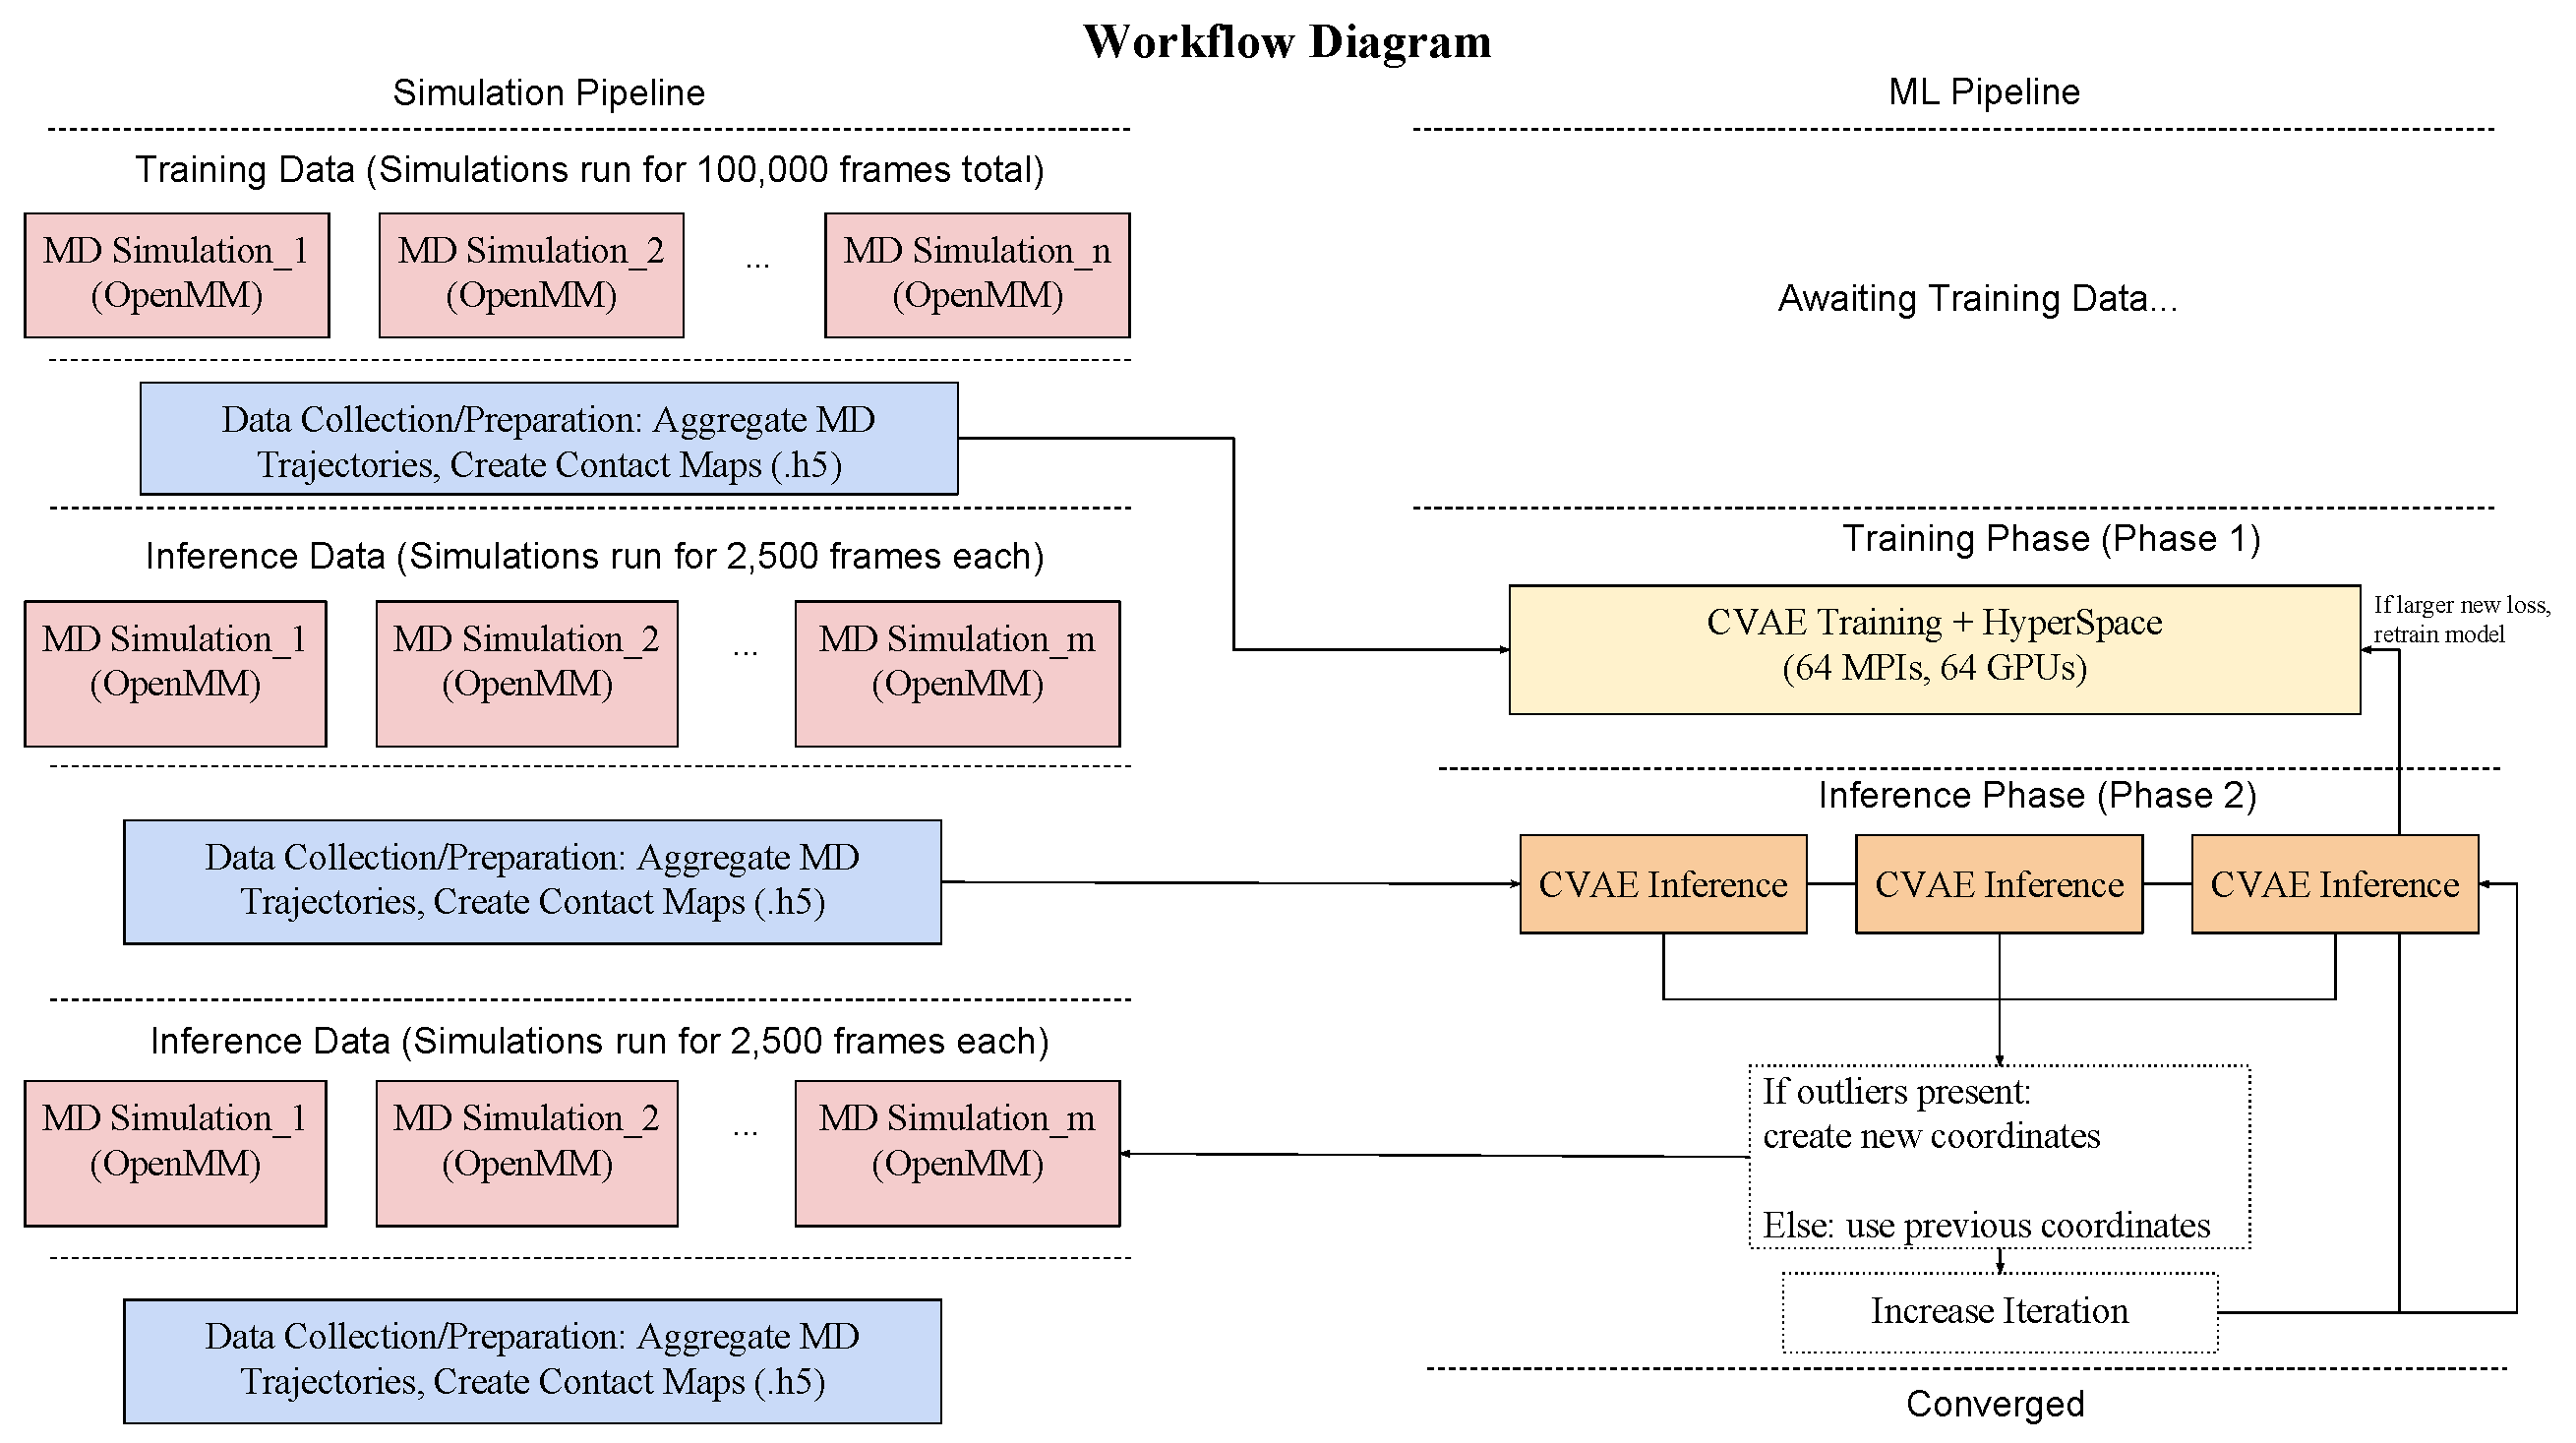
\includegraphics[width=.8\textwidth]{MicroScope_Workflow_Diagram}
	\caption{The workflow diagram. Each frame in MD simulations is equivalent to 50 ps. }
	\label{fig:microscopeworkflowdiagram}
\end{figure*}
% ---------------------------------------------------------------------------
\section{Software and Platforms}

EnTK exposed an application programming interfaces that enables users to
specify workflows in terms of pipelines, stages and tasks. Each pipeline is
composed by a sequences of stages and each stage is a set of tasks. Sequences
and set encode the execution priority among tasks: stage \#2 must execute
after stage \#1 but all tasks of each stage can execute concurrently. Each
task encapsulates a program, not a method or a function. We use the OpenMM
simulation engine to execute our MD simulations. Each OpenMM executable runs
on a single GPU and simulates an independent physical system. Each OpenMM
executable and CVAE is run as a self-contained, independent executable that,
in turn, can use multithreading and/or multiprocessing. In this way, each
task can use multiple CPUs or GPUs as needed.

EnTK uses RADICAL-Pilot (RP) as its runtime system~\cite{merzky2018using}. RP
is a pilot systems, i.e., it enables the decoupling between the acquisition
of HPC resources and the scheduling of tasks on those
resources~\cite{turilli2018comprehensive}. RP acquires resources by
submitting a job to the batch system of the target resource and then uses a
private scheduler to schedule tasks on those resources. In this way, tasks do
not have to wait on the resource batch queue to be executed, enabling
high-throughput on high-performance computing resources within the boundaries
of the fair usage policies of the target machine.

We executed our workflow on Summit, the new leadership-class machine managed
by OLCF at ORNL\@. Currently, Summit is the largest HPC machine in the world,
offering 44 CPU cores and 6 GPUs per node.


% ---------------------------------------------------------------------------
\section{Results and Future Work}

Our workflow uses 18 concurrent OpenMM instances and requires 18 GPUs. Once
we execute all OpenMM instances we aggregate all simulation results and pass
them to a CVAE task that uses these results to train a CVAE model. 

We show preliminary results that indicates the ability to integrate the 
simulation component of the workflow into RADICAL-Cybertools.  We profile the 
performance of RADICAL-Cybertools using a single OpenMM instance on ORNL Summit. 
Specifically, we benchmark the FS-Peptide system and run the 
simulations for 100 nanoseconds (ns) on a single Tesla V100 GPU. We include the 
overheads of EnTK and RP, using our in-house profiling tool (RADICAL-Analytics). 
In addition, we include the task execution time reported by the OpenMM logs. 
% Performance of RADICAL-Cybertools using 
    % FS-Peptide OpenMM benchmark on ORNL Summit
\begin{figure*}
    \centering
    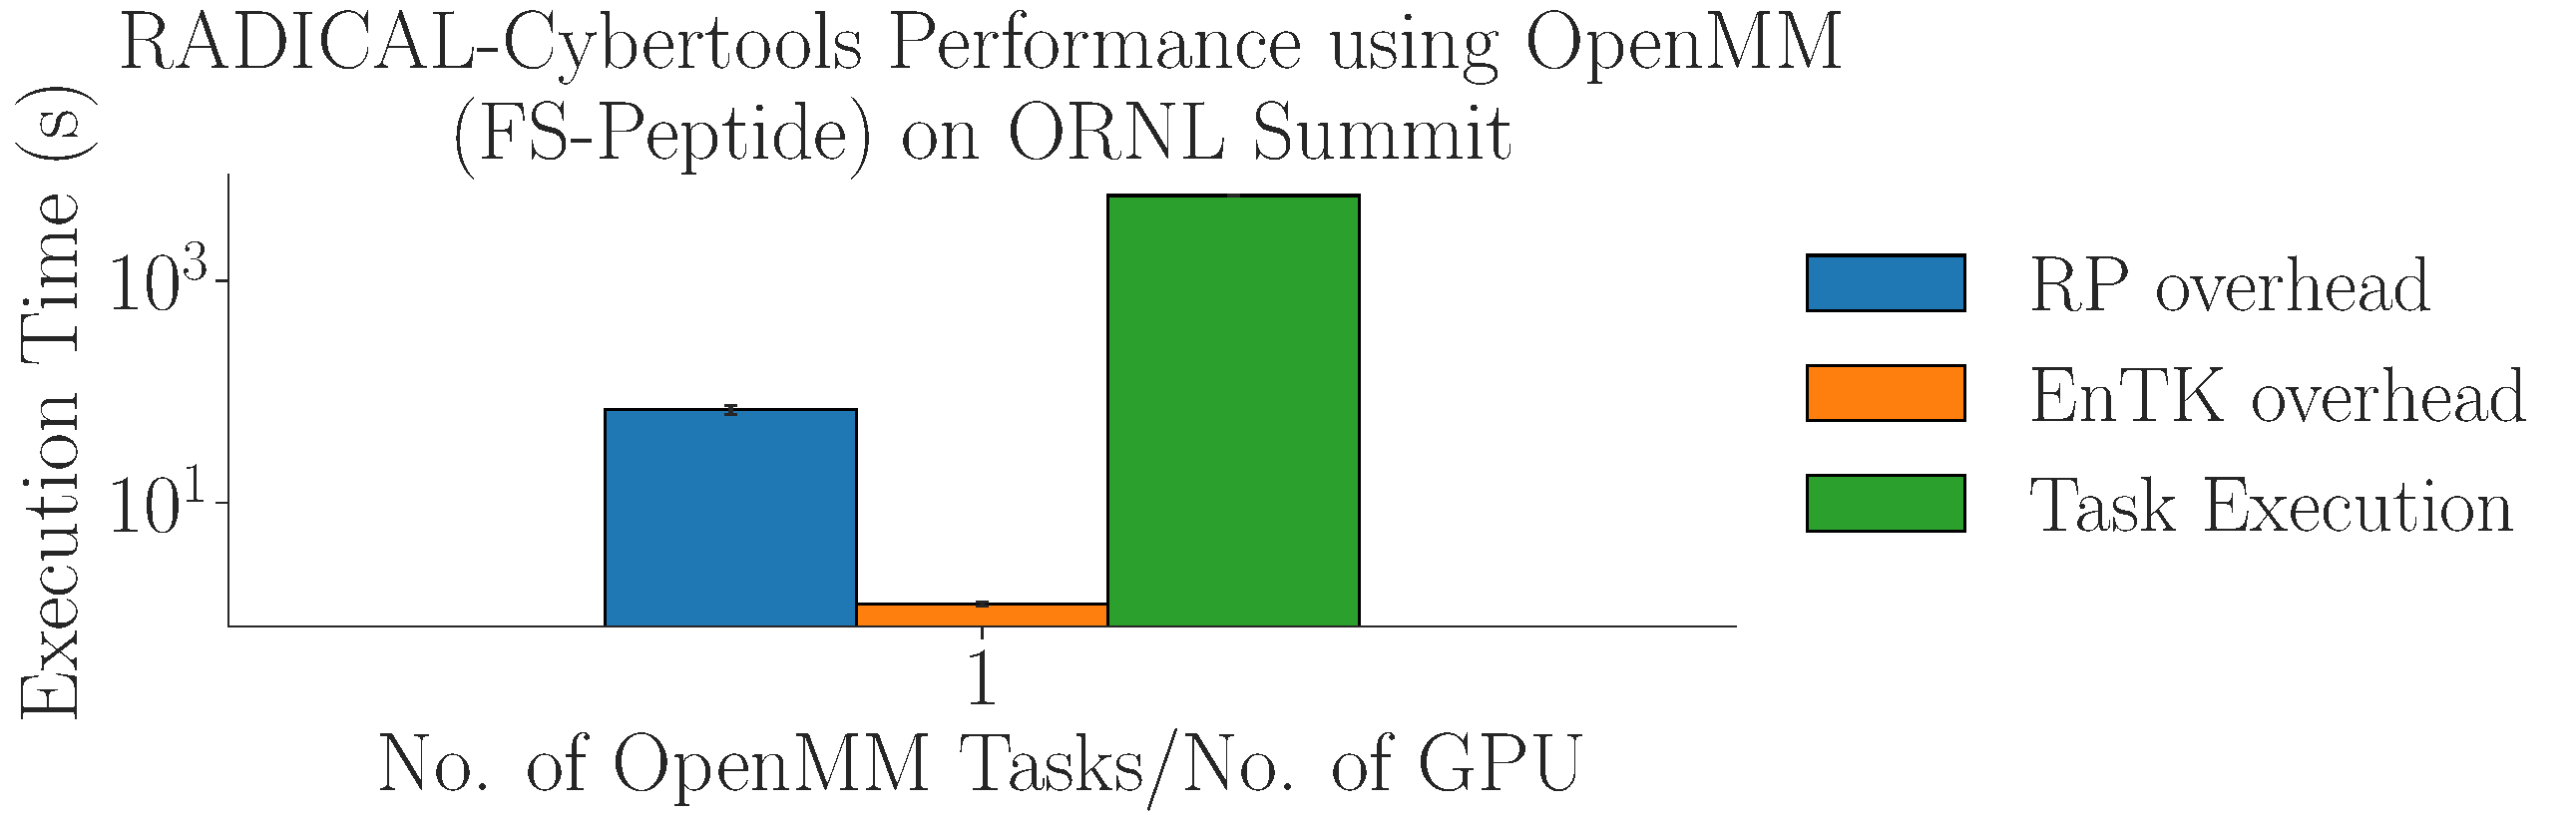
\includegraphics[width=.8\textwidth]{single_openmm}
    \caption{}
    \label{fig:single_openmm}
\end{figure*}



\bibliographystyle{unsrt}
\bibliography{parco-micro}

\end{document}